\chapter{Pre-selection optimisation based on \texorpdfstring{$\frac{\mathsf{S}}{\sqrt{\mathsf{S}+\mathsf{B}}}$}{S/sqrt(S+B)}}\label{sec:appendix_sqrtsplusb_optimisation}

To validate figure-of-merit $\mathrm{FOM}_2$ defined in \Cref{eq:punzi_fom}, the same optimisation is performed based on the more-standardised $\mathrm{FOM}_1$ defined in \Cref{eq:soversqrtsplusb}.
In general, this would be expected to provide an equivalent result.
This is shown in \Cref{fig:selection_optimisations_sqrtsplusb}.
The Figure is equivalent to \Cref{fig:selection_optimisations} with a different figure-of-merit in mind.
As can be seen, consistent conclusions with \Cref{sec:preselection} can be drawn.
Therefore, in this analysis $\mathrm{FOM}_2$ is chosen due to the advantages discussed in the main body of the thesis.

\begin{figure}[htbp!]
    \centering
    \subcaptionbox{\label{fig:bp_zmva_optimisation_sqrtsplusb}}{
            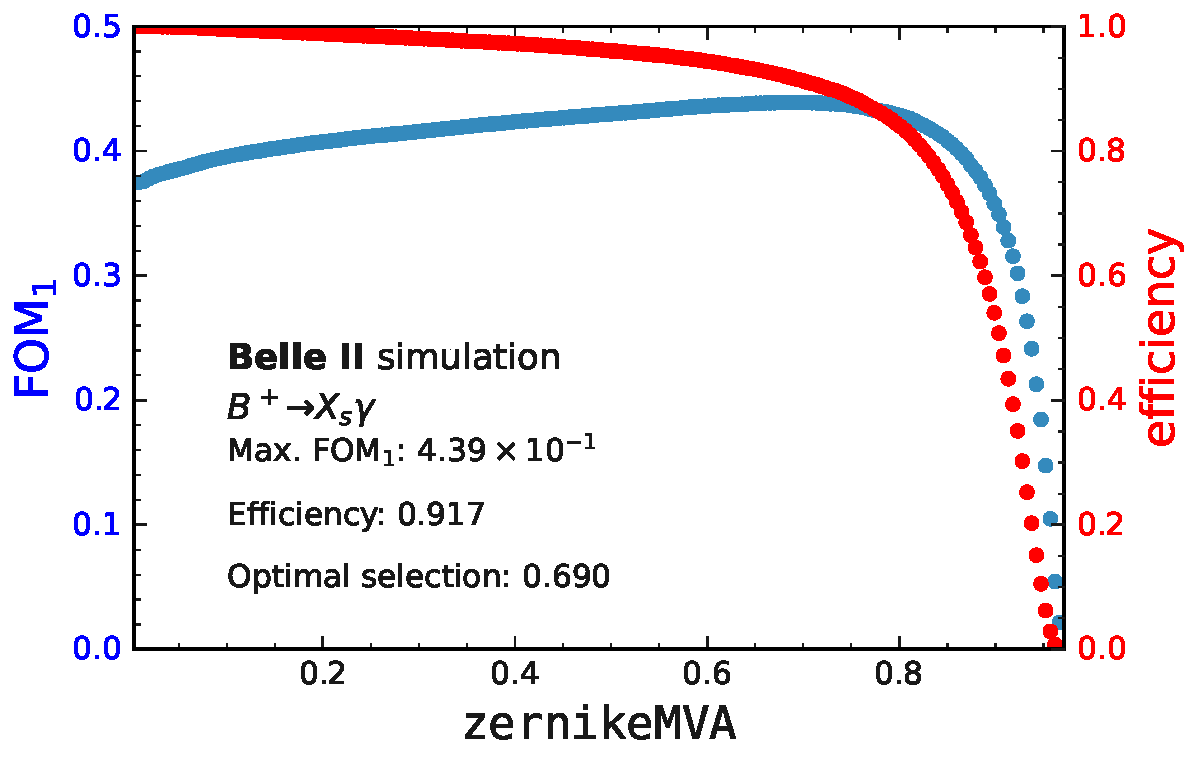
\includegraphics[width=0.3\textwidth]{figures/continuum_suppression/Bp_zernikeMVA_optimisation_sqrtsplusb.pdf}
        }
    \subcaptionbox{\label{fig:bp_piveto_optimisation_sqrtsplusb}}{
            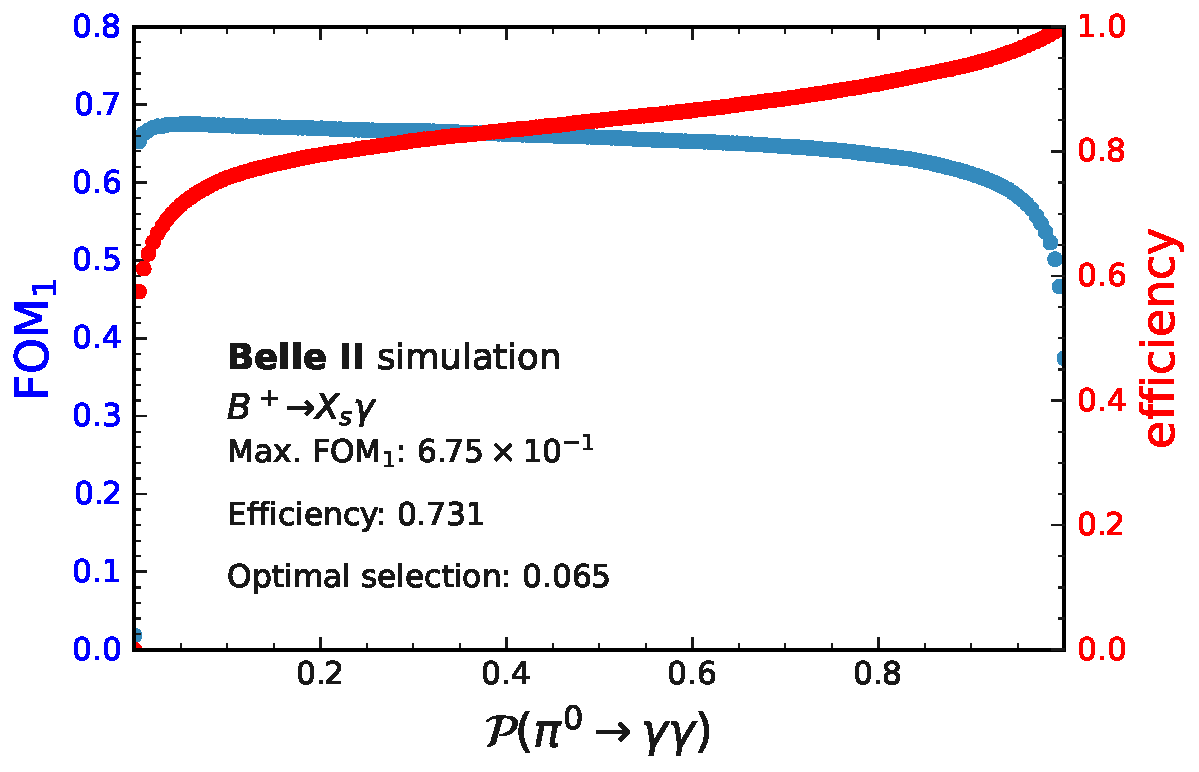
\includegraphics[width=0.3\textwidth]{figures/continuum_suppression/Bp_piVeto_optimisation_sqrtsplusb.pdf}
        }
    \subcaptionbox{\label{fig:bp_etaveto_optimisation_sqrtsplusb}}{
            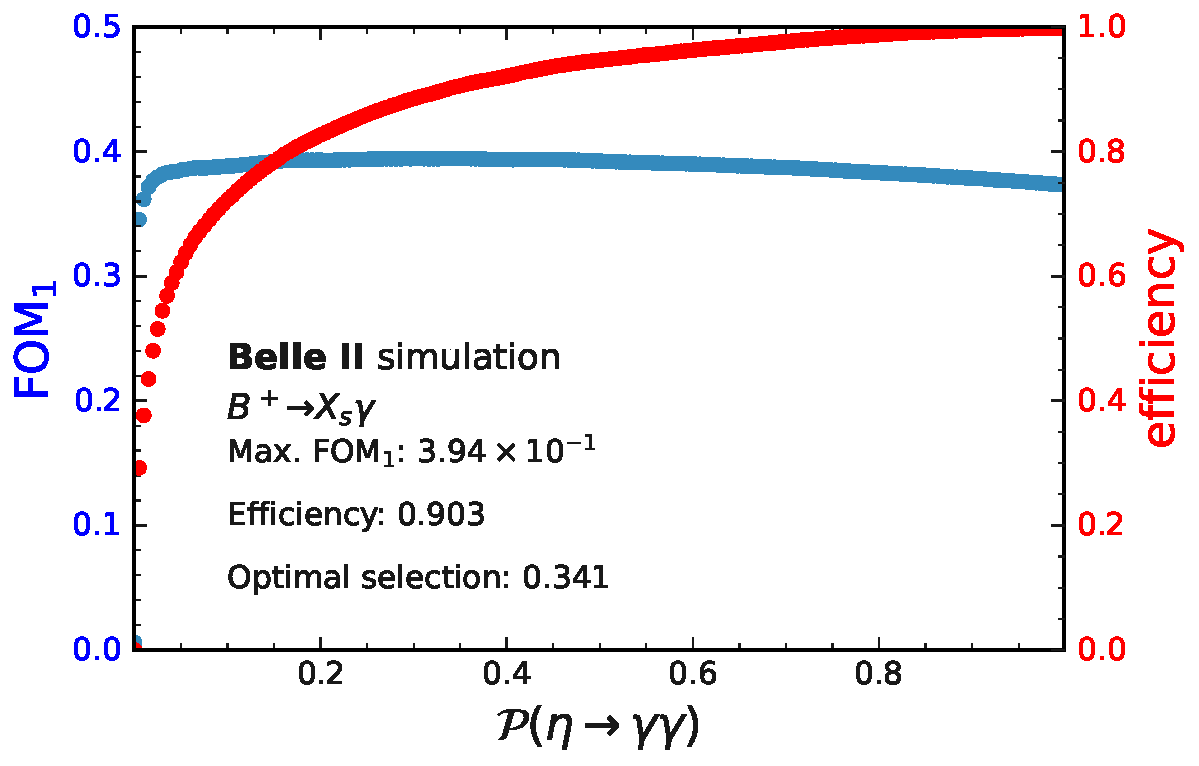
\includegraphics[width=0.3\textwidth]{figures/continuum_suppression/Bp_etaVeto_optimisation_sqrtsplusb.pdf}
        }
    \subcaptionbox{\label{fig:bz_zmva_optimisation_sqrtsplusb}}{
            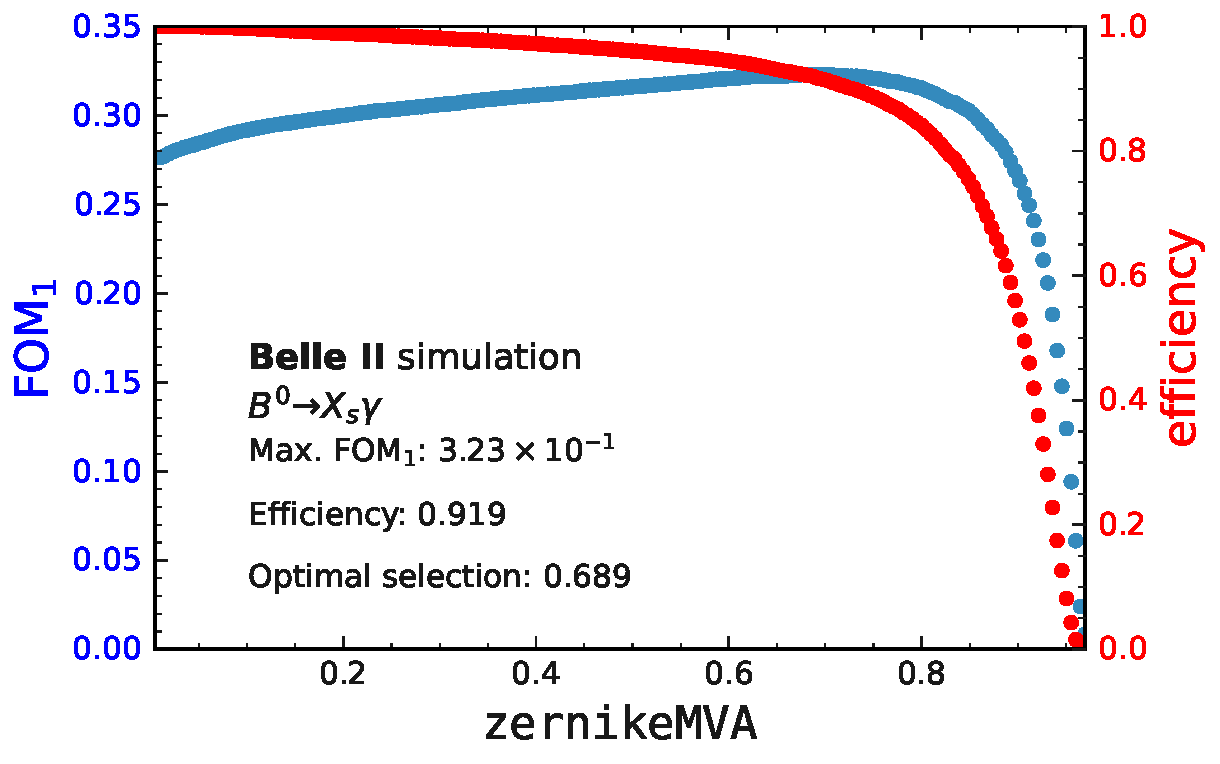
\includegraphics[width=0.3\textwidth]{figures/continuum_suppression/Bz_zernikeMVA_optimisation_sqrtsplusb.pdf}
        }
    \subcaptionbox{\label{fig:bz_piveto_optimisation_sqrtsplusb}}{
            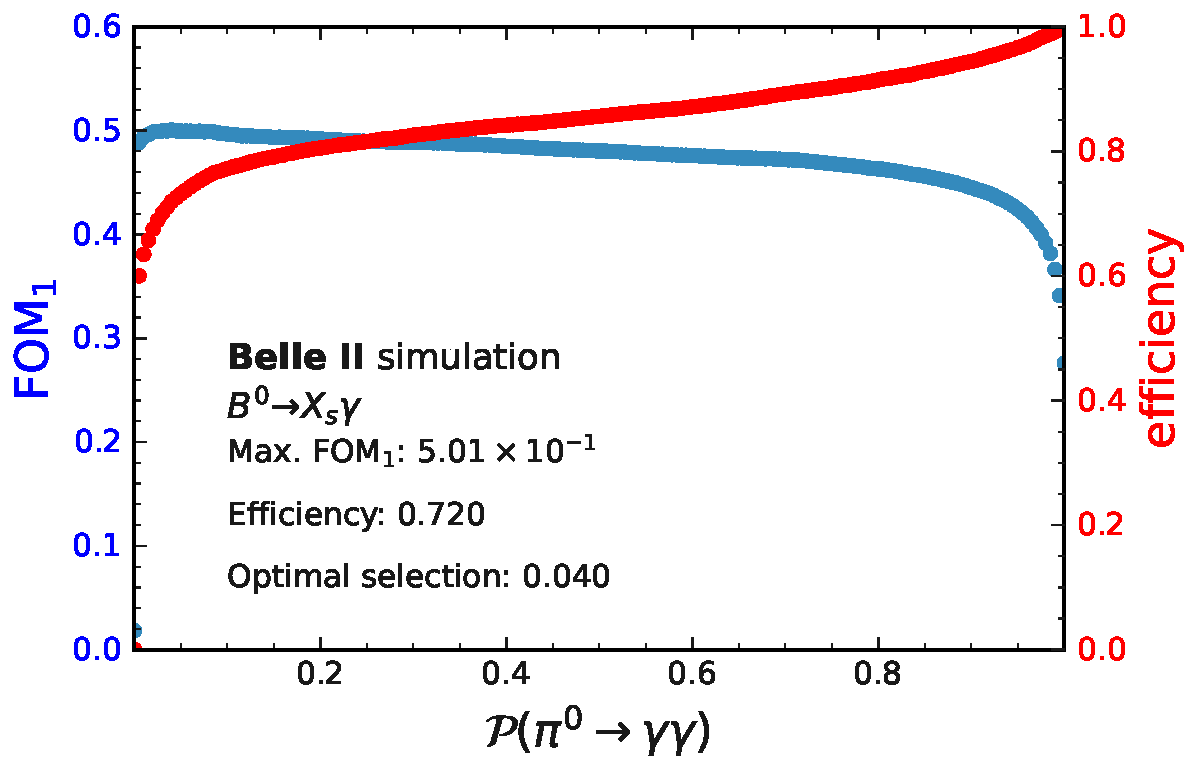
\includegraphics[width=0.3\textwidth]{figures/continuum_suppression/Bz_piVeto_optimisation_sqrtsplusb.pdf}
        }
    \subcaptionbox{\label{fig:bz_etaveto_optimisation_sqrtsplusb}}{
            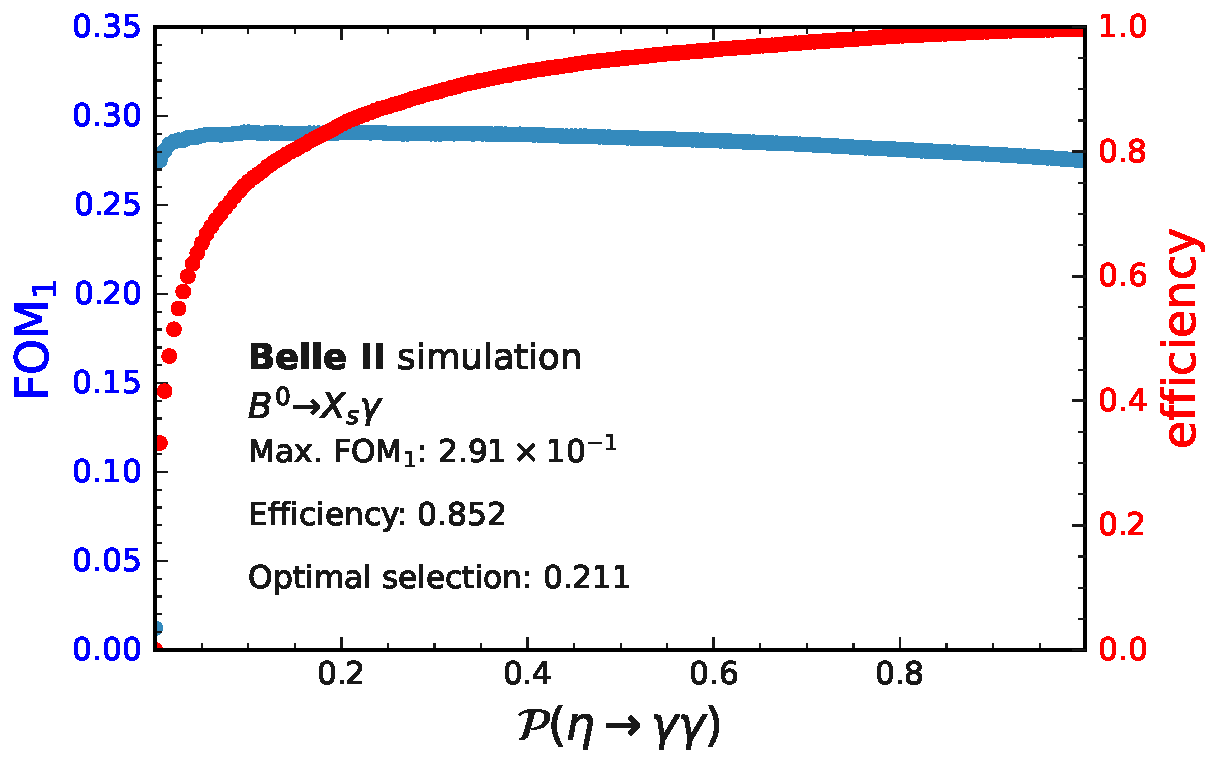
\includegraphics[width=0.3\textwidth]{figures/continuum_suppression/Bz_etaVeto_optimisation_sqrtsplusb.pdf}
        }
    \caption{\label{fig:selection_optimisations_sqrtsplusb} Optimal selection calculation for observables
    described in \Cref{sec:photon_selection} based on $\mathrm{FOM}_1$ (see \Cref{eq:soversqrtsplusb}).
    For \BptoXsgamma events the tests are shown
    in \Cref{fig:bp_zmva_optimisation_sqrtsplusb,fig:bp_piveto_optimisation_sqrtsplusb,fig:bp_etaveto_optimisation_sqrtsplusb},
    and for \BztoXsgamma in \Cref{fig:bz_zmva_optimisation_sqrtsplusb,fig:bz_piveto_optimisation_sqrtsplusb,fig:bz_etaveto_optimisation_sqrtsplusb}.
    The figures show the efficiency and $\mathrm{FOM}_1$ score calculated for 200 selections of \piVeto, \etaVeto and \ZMVA.
    The maximum value of $\mathrm{FOM}_1$, the corresponding selection and efficiency are shown as well.
    }
\end{figure}
